
\chapter{Typological comparison of marked"=S languages}\label{typology}

\section{Introduction}

In the previous chapters I have presented an in-depth investigation of the coding patters of a number of S-like roles (and other roles commonly associated with the nominative case in standard nominative"=accusative languages) in marked"=S languages. 
Nominal case-marking, and more precisely the contrast between overtly coded forms and zero-coded forms, has been the central aspect of what I have called the `micro-alignment' system of these languages.
In this chapter, I will employ the data collected in the individual chapters in order to produce two typologies. 
First, I will compare the data based on the different roles that I have investigated. 
For each of these roles the extent to which they behave like regular S arguments will be investigated.
The other base of comparison is the language (and genus) level. 
In this typology of marked"=S languages I will compare how similar the languages of this type behave with respect to one another. 
It will also be investigated whether distinct subtypes of marked"=S languages can be identified.
Based on this data, %I will compare the two different definitions of marked"=S languages, the formal and the functional one as discussed in Chapter 1. And also 
the difference between the weak and strong form (cf. Section~\ref{functional}) of the functional marked"=S hypothesis by \citet{Koenig:2006} will be put to a test.

In Section \ref{general} I give a brief discussion on the nature of typological comparisons with focus on the statistical validity of the results.
Also, information is provided on how the data has been organized for the typological interpretation in the following sections.
Afterwards, the data collected in this study will be compared on the basis of the roles that were studies (Section \ref{rolestyp}). 
Following this, the data will be presented from point of view of the individual languages (Section \ref{languagestyp}). 
At least the marked"=S languages of North America appear to form a distinct subtype, which behaves differently from the well-known marked"=S languages of East Africa. 
While the first two data analysis sections present the data in the form of numbers and percentages in the form of ranked tables, Section \ref{networkstyp} uses phylogenetic networks\is{phylogenetic networks} produced with the NeighborNet\is{NeighborNet} algorithm \citep{NeighborNet} for visualization.
Section \ref{area} provides a discussion of the geography of the marked"=S type of coding. 
The languages of my sample are located in three macro-areas\is{typology!areal}: North-East Africa, the North American West Coast, and the Pacific. 
For each of these macro-areas, the influence that genealogy and areal proximity could have had on the development of the rare marked"=S type of language are discussed.
Finally, the findings are summarized in Section \ref{sumtyp}.
     

\section{Making generalizations}\label{general}

Traditional large scale typologies attempt to make statements about the world-wide distribution of certain linguistic features.
These distributions can then be used to arrive at cross-linguistic generalizations and to describe general tendencies of linguistic behavior.
The nature of this study  does not allow for a classical typological sample that is balanced for areal and genealogical affiliation. 
The phenomenon studied is known to be extremely rare on a world-wide basis and geographically highly skewed.
Given the rarity of the phenomenon of marked"=S coding, the primary goal of this study has instead been to collect data from as many languages exhibiting this pattern as possible. 
In the previous chapters (\ref{nompred}--\ref{extrasyn}) all marked"=S languages for which data on one of the roles was available have been included into the discussion. 
For a number of languages, only very few of the roles studied were represented in the available data. 
This has not been a problem, given the more descriptive nature of these chapters. 
However, large sets of missing data are problematic for making typological generalizations and for statistical analysis of the data. 
Therefore not all languages mentioned before will be included in the following analysis. 

\begin{figure}[h,t,b] \centering \resizebox{\textwidth}{!}{\fbox{
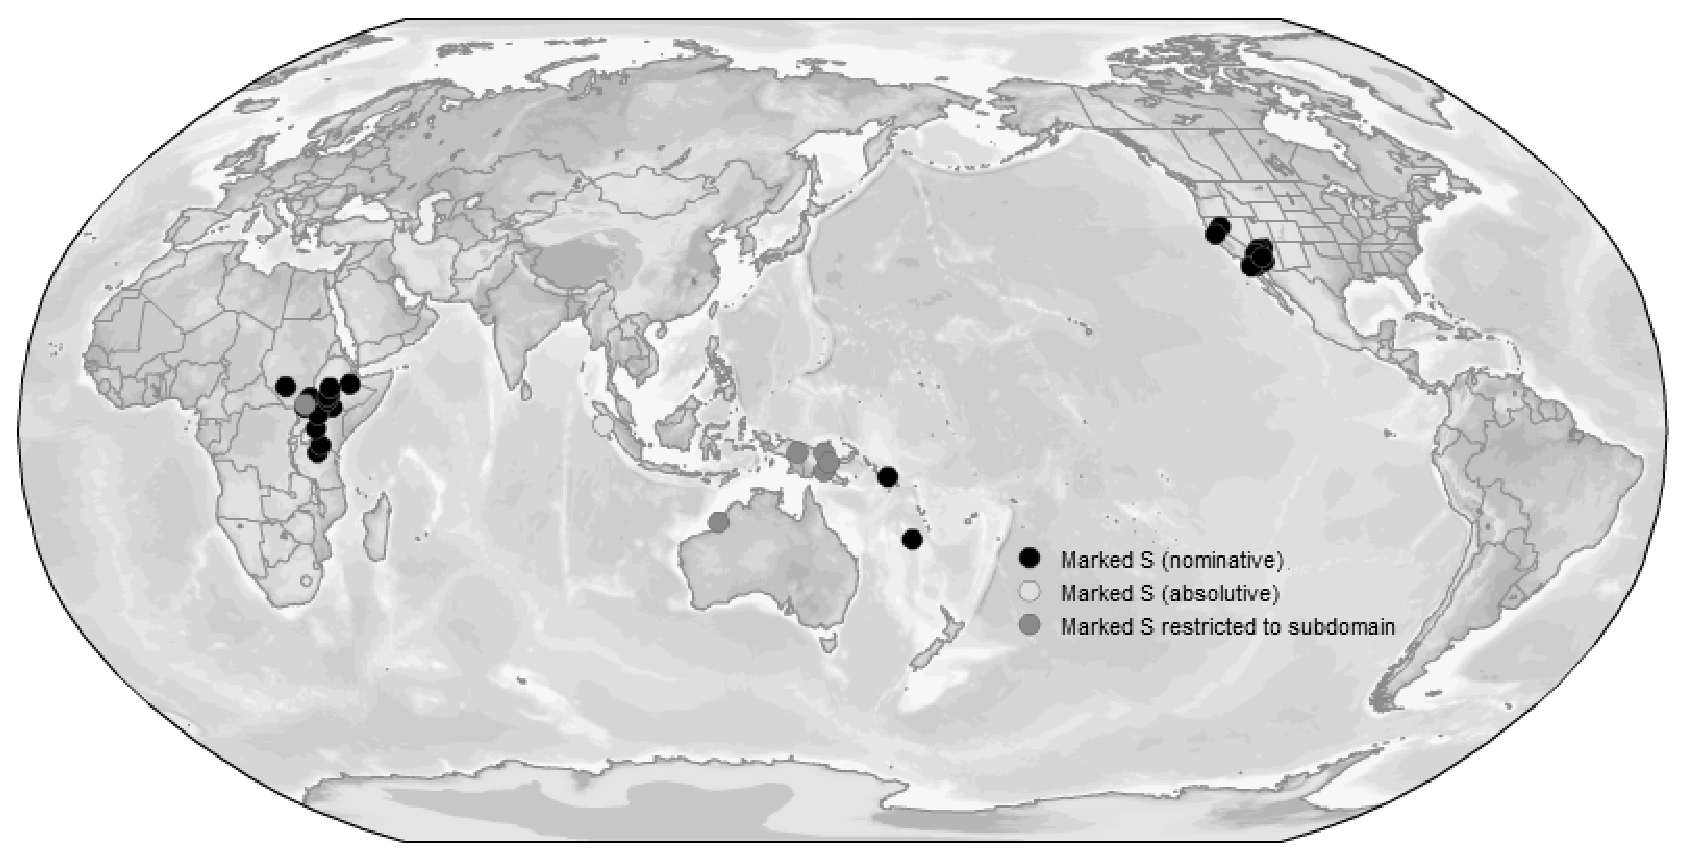
\includegraphics[scale=0.45]{MapFullABW}
}}
\caption{Distribution of the languages studied in Chapters 3--7}\label{MapFullBW}
\end{figure}

%An overview table summarizing all roles discussed in this study and all languages is provided at the end of this chapter. 
Figure~\ref{MapFullBW} shows the distribution of all languages that have been discussed at some stage in Chapters \ref{nompred} to \ref{extrasyn}.
\footnote{The maps shown in this chapter were generated with the interactive tool of the \textit{World Atlas of Language Structures} \citep{WALS}, which was developed by Hans-J\"org Bibiko.} 
Out of these 33 languages, ten languages have data for less than half of the  roles on which data has been collected (the number of roles studied is 17 in total, including the transitive roles of A and P). 
These languages are not included in the following.
\footnote{The languages which have been excluded from the analysis in the present chapter are all of the Pacific languages with the marked"=S pattern only for emphatic\is{emphatic subject} subjects discussed in Chapter \ref{emphaticS}, namely Eipo\il{Eipo}, Kaki Ae\il{Kaki Ae}, Nabak\il{Nabak}, Waskia\il{Waskia} and Yawuru\il{Yawuru}. In addition, the Yuman languages Cocopa\il{Cocopa}, Maricopa\il{Maricopa} and Walapai\il{Walapai} have been excluded due to lack of data, as well as the Nilotic languages P\"ari\il{P\"ari}, which has the marked"=S pattern only in some non-basic clauses, and Dinka\il{Dinka (Agar)}.} 
The remaining 23 languages are visualized on the map in Figure \ref{MapReduxBW}.

\begin{figure}[htbp] \centering \resizebox{\textwidth}{!}{\fbox{
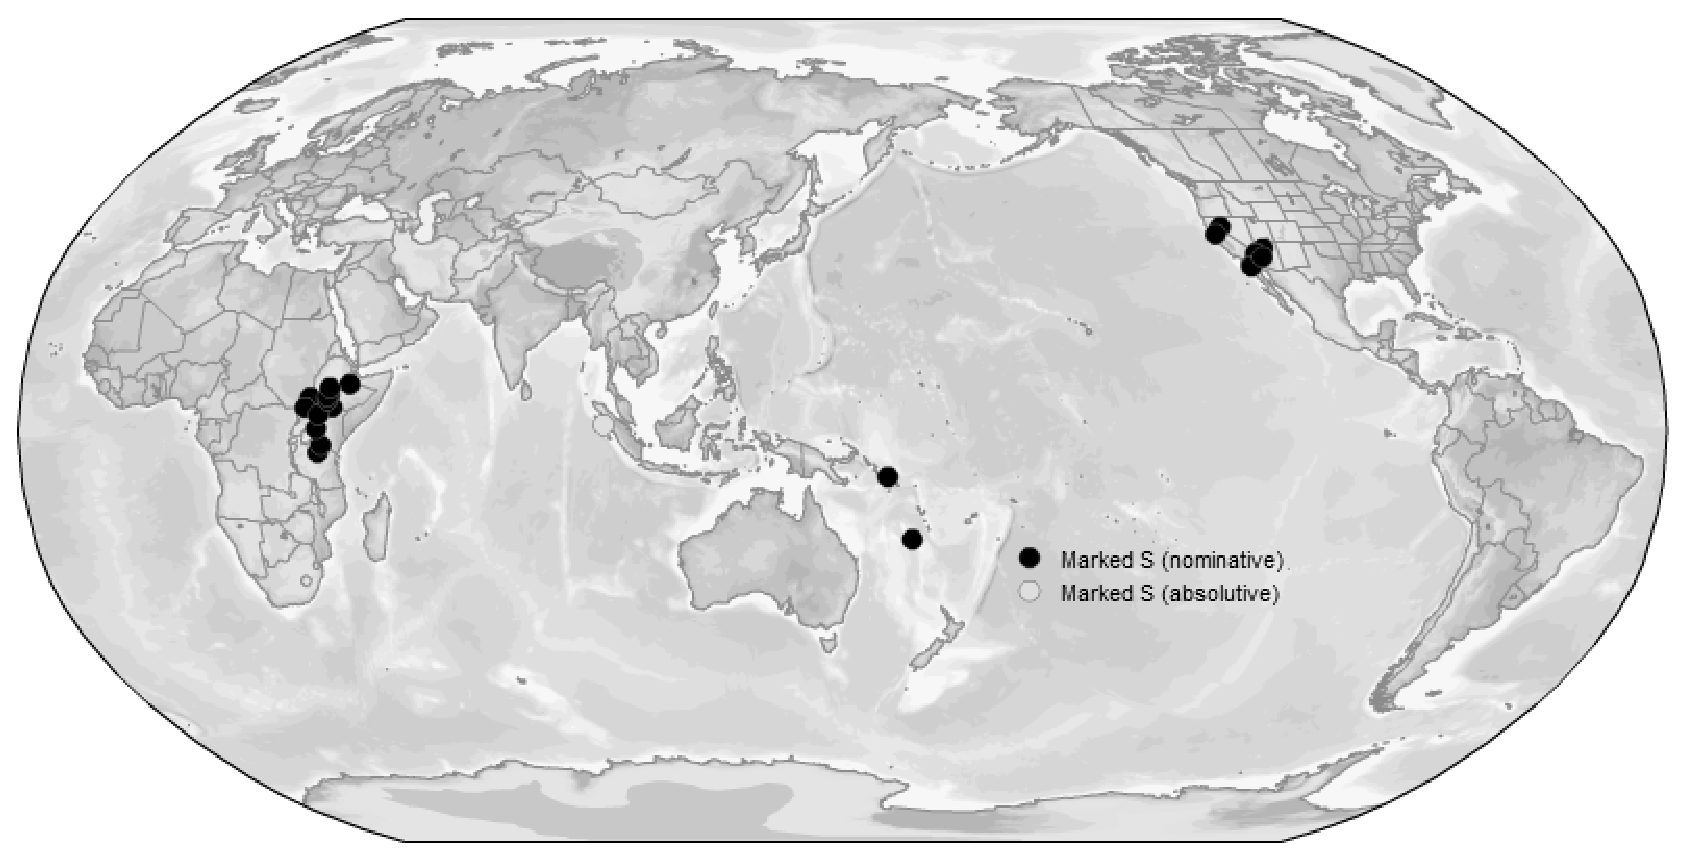
\includegraphics[scale=0.45]{MapReduxBW}}
}
\caption{Distribution of the languages used for comparison}\label{MapReduxBW}
\end{figure}


The data collected in this study provides information on the encoding of individual roles in individual languages. 
Both types of entities, i.e. roles and languages, can be used as the means of comparison, and indeed both will be used in the next sections.
In the remainder of this section I will discuss the two means of comparison. 
The language level will be discussed first, followed by the role level. 

When\is{typology!sampling!genealogical grouping|(} making typological generalizations over a number of languages, one runs into a problem when trying to arrive at meaningful results.
Statistical analysis of the data demands independence of the data. 
This criterion is, however, not necessarily met by language data that comes from related languages; and, as \citet{Dryer:1989} remarks, all languages in the world might well be related to one another.
If a sample of languages contains a large number of related languages sharing a linguistic feature (potentially due to their common origin), this feature might wrongly be shown to be a significantly preferred across the world's languages, though in fact this preference only holds for the respective genealogical grouping. 
This and related problems are discussed in \citet{Dryer:1989} and \citet{Bickel.samp}; these two papers also propose solutions on how to avoid misinterpretation of typological preferences.
In short, the suggested solutions propose genealogical (and also areal) control of samples, even though if taken to the extreme, this procedure can lead to very small sample sizes, leading to other statistical difficulties. 

Two questions arise when attempting to balance data sets according to genealogy (and areal distribution).
First, between which groupings of languages can relative independence of the data be expected, and second, how does one then proceed to balance the data between those groupings in the analysis.
\citet[267]{Dryer:1989} proposes the genus as the level of relatedness above which one can assume relative independence of data points, though he notes that different linguistic features have different levels of stability and therefore some features might be considered independent on a smaller or larger time scale. 
Accordingly, with this the data will be analyzed on the genus level in addition to the analysis based on individual languages.
The genera used in this study are taken from the classification used in \citet{WALS}. 
Different methods are available to balance the data with respect to the groups one has established for the analysis. 
The first possibility is to pick a representative language for each of the defined groups and use the data of this language. 
However, based on the language choice, the data representing a group of languages might not be representative for the group as a whole.
Another possibility is to include more languages for each group in order to take into account in-group variation but to weight the data of the individual groups with respect to each other in the later analysis. This procedure provides `controlled genealogical sampling' \citep{Bickel.samp}. 
I have chosen a similar method for analyzing marked"=S languages on a genealogically controlled level (though the details differ from \citeauthor{Bickel.samp}'s proposal). 
For each role that is investigated, an average figure of the encoding-pattern has been calculated based on the languages of the respective genealogical grouping. 
The same has also been done to determine the coding-pattern of the individual languages in case they allow for alternative constructions to encode a certain role. 
Both types of data, based on individual language data and grouped genealogically, are presented in the following, and the results are compared.\is{typology!sampling!genealogical grouping|)}
 
In addition to the distinction between the level of individual languages and genus, another contrast is made in my analysis of marked"=S languages.
For each dataset, I provide two types of coding. 
In Section~\ref{explain}, I\is{marked-S languages!functional definition!strong versus weak hypothesis|(} have distinguished between the weak and strong version of the functional explanation of marked"=S. 
In general, the functional hypothesis proposed by \citet{Koenig:2006} lessens the impact of the marking of the S, A and P roles. 
It takes other roles into consideration and states that the overall distribution of the less-coded form (the zero-case in my terminology) should have a wider distribution as the form it corresponds to with respect to the S, A and P encoding would have in non-marked"=S languages. 
What exactly is meant by wider distribution is, however, left a bit vague. 
Two possible interpretations are, first, that the zero-case is used in more contexts than the S-case (weak version) or, second, that the zero-case is used in more contexts than all other (overt) case-forms together (strong version). 
In accordance with these two versions of the hypothesis, I have compared two different encodings of the role-encoding data in marked"=S languages. 
In the first variant, I code whether a role is encoded by the same case-form as the prototypical P or A role (dubbed the zero-case in this study), or as the S+A/P role.
In addition, roles that are coded by neither of the two case-forms are listed in a separate column as `other'. 
The second coding used for the data strictly distinguishes whether a role is encoded by zero-coding or by overt material. 
For many roles, the second coding can be derived from the first coding by adding up the S-case and other case columns. 
However, the zero- versus overt-coding data-representation also includes forms of overt coding other than case-marking.
For example, the genitive particles found in the attributive\is{possession!attributive} possessive construction in many languages (cf. Chapter~\ref{extrasyn}) are represented as overt material.\is{marked-S languages!functional definition!strong versus weak hypothesis|)}

\section{Comparison across roles}\label{rolestyp}

The roles studied in the previous chapters show varying tendencies of behavior similar or dissimilar to that of S arguments in terms or their overt coding.
While all of the roles are found to be encoded with the S-case in at least one language of my sample, the proportions of S-like and non-S-like encoding exhibit wide variation between the individual roles. 
While subjects of locational\is{locational predication} clauses are almost always encoded like standard intransitive subjects of a language, the form used in citation\is{citation form} is only encoded in this way as an alternative strategy in one language, namely Nias\il{Nias} (a behavior that most likely is a very recent innovation).  
Further, for the roles investigated, if a case-form other than the S-case is chosen, then the zero-case is the most likely alternative, although this varies between the roles, too. 
For attributive\is{possession!attributive} possessors, the tendency to choose the zero-coded case is equally strong as the tendency to employ a special overtly coded case-form, a genitive. 
These findings apply to the total set of individual languages as well as to a genealogically controlled sample.
In this section I will discuss these results in more detail. 

%language level, roles as coded by case function (S,A,P other)
 
\begin{table}[h,t,b]
\begin{center}
\caption{Overview on percentage of zero-case and S-case-marking for different roles}\label{SumRoleLang}
\begin{tabular}{lccccccc}
\hline \hline
\bfseries role &\multicolumn{2}{c}{\bfseries $\emptyset$-case} &\multicolumn{2}{c}{\bfseries S-case} &\multicolumn{2}{c}{\bfseries other}&\bfseries total \\
{}&No.&\%&No.&\%&No.&\%& \bfseries languages\\
\hline
S argument &0  &0\,\% &23  &100\,\%  &0  &0\,\% & 23\\
%\hdashline
Locational S &0.5  &2\,\% &21.5  &98\,\% &0  &0\,\% &22\\
%\hdashline
%%%S VIC&1  &7\,\% &13  &93\,\% &0  &0\,\% &14\\
%%%%% \hdashline
S VDC&3.5  &23\,\%  &11.5  &77\,\% &0  &0\,\% &15\\
%\hdashline
Positive existentials&4.5  &23\,\% &14.5  &73\,\% &1  &5\,\% &20\\
%\hdashline
Adverbial clauses&2  &22\,\% &6.5  &72\,\% &0.5  &6\,\% &9\\
%\hdashline
Nominal predication&7  &33\,\% &14  &67\,\% &0  &0\,\% &21\\
%\hdashline
Negative existentials&4  &40\,\% &6  &60\,\% &0  &0\,\% &10\\
%\hdashline
Relative clauses&6  &35\,\% &10  &59\,\% &1  &6\,\% &17\\
%\hdashline
Emphatic S&7  &41\,\% &8  &47\,\% &2  &12\,\% &17\\
%\hdashline
Complement clause&3  &60\,\% &2  &40\,\% &0  &0\,\% &5\\
%\hdashline
Predicate nominal&17  &77\,\% &4  &18\,\% &1  &5\,\% &22\\
%\hdashline
Term of address&8.5  &65\%  &0.5  &4\% &4  &31\% &13\\
%\hdashline
Attributive possessor&10  &43.5\,\%  &1  &4\,\% &12  &52\,\% &23\\
%\hdashline
Citation form&22.5  &98\,\% &0.5  &2\,\% &0  &0\,\% &23\\
\hline \hline
\end{tabular}
\end{center}
\end{table}

Table~\ref{SumRoleLang} lists the roles studied. 
For each role, it is indicated which percentage of the languages uses a certain case-form. 
Three different case values are distinguished, namely the zero-case, the S-case and other, if a different case-form altogether is used for the respective role. 
If a language uses more than one strategy for a role, both patterns are included and a mean score from all different constructions is listed for the encoding of the role. 
If, for example, a language has two constructions that encode a context and the relevant role is encoded using the S-case in the first construction and the zero-case in the second construction, this role is represented with the value 0.5 in both columns.  
The roles are listed in decreasing order according to the percentage the S-case is used for encoding.
\footnote{The percentages have been rounded to full integers in the following. Therefore, the values in one row of the table add up to 101\,\% instead of 100\,\% for some rows.}

The data in table~\ref{SumRoleLang} show that the role that behaves most like intransitive S arguments in terms of overt coding is the subject of locational\is{locational predication} clauses. 
This role is marked with the S case in 98\,\% of the languages, while it is encoded with the zero case in only 2\,\%. 
On the other end of the scale is the citation form\is{citation form} of a noun. 
Figures for this role are the reverse of those of the locational\is{locational predication} subject, with 2\,\% being encoded with the S-case and 98\,\% with the zero-case. 
In between these two extremes, the other roles line up. 
The non-clause-level roles all have percentages below five for the S-case encoding, but they still differ in their encoding behavior. 
While the citation\is{citation form} form, as mentioned above, almost exclusively makes use of the zero-case, half of the attributive\is{possession!attributive} possessors are encoded by a different case-form altogether, and roughly the other half is encoded by the zero-case. 
Terms of address\is{terms of address} are located in between these to patterns with roughly a third of the languages using a different case-form altogether, and about two thirds using the zero-case. 
 
There are a number of roles that behave more like intransitive S arguments in terms of their encoding.
In addition to subjects of locational\is{locational predication} clauses, most roles that will be subsumed under the subject category in most grammars are encoded like intransitive S arguments quite regularly. Subjects of %valency-increasing (93\,\%) and 
valency-decreasing\is{valency-decreasing construction} constructions (77\,\%), positive existential\is{existential predication} constructions (73\,\%), adverbial clauses (72\,\%) and nominal predications\is{nominal predication!subject of} (67\,\%) are regularly marked with the same case as prototypical S arguments in two thirds of the languages in the sample or more. 
Negative existential constructions\is{existential predication} (60\,\%) and relative clauses (59\,\%) still use the S-case in more than half of the cases. 
Emphatic\is{emphatic subject} subjects (47\,\%) and complement clauses (40\,\%) are encoded like typical S arguments in just below fifty percent of the languages.
Finally, predicate nominals\is{nominal predication!predicate nominal} (18\,\%) are seldom encoded in the S-case in marked"=S languages. 
This role is similar to the non-clause-level roles since it does not represent a type of subject.

%language level, roles compared by coding (overt/ zero)

\begin{table}[h,t,b]
\begin{center}
\caption{Overview on percentage of zero versus overt coding for different roles}\label{SumRoleLangZero}
\begin{tabular}{lccccc}
\hline \hline
\bfseries role &\multicolumn{2}{c}{\bfseries zero-coding} &\multicolumn{2}{c}{\bfseries overt coding} &\bfseries total \\
{}& No.&\%&No.&\%& \bfseries languages\\
\hline
S argument &0  &0\,\% &23  &100\,\%  & 23\\
%\hdashline
Locational S &0.5  &2\,\% &21.5  &98\,\% &22\\
%\hdashline
%%%%%%S VIC&1  &7\,\% &13  &93\,\% &14\\
%%%%%%% \hdashline
S VDC&2.5  &17\,\%  &12.5  &83\,\% &15\\
%\hdashline
Adverbial clauses&2  &2\,\% &7  &78\,\% &9\\
%\hdashline
Positive existentials&4.5  &23\,\% &15.5  &78\,\% &20\\
%\hdashline
Emphatic S&5  &29\,\% &12  &71\,\% &17\\
%\hdashline
Nominal predication&7  &33\,\% &14  &67\,\% &21\\
%\hdashline
Relative clauses&6  &35\,\% &11  &65\,\% &17\\
%\hdashline
Negative existentials&4  &40\,\% &6  &60\,\% &10\\
%\hdashline
Attributive possessor&10  &43\,\%  &13  &57\,\% &23\\
%\hdashline
Complement clause&3  &60\,\% &2  &40\,\% &5\\
%\hdashline
Term of address&8.5  &65\,\%  &4.5  &35\,\% &13\\
%\hdashline
Predicate nominal&17  &77\,\% &5  &23\,\% &22\\
%\hdashline
Citation form&22.5  &98\,\% &0.5  &2\,\% &23\\
\hline \hline
\end{tabular}
\end{center}
\end{table}

Table~\ref{SumRoleLangZero} distinguishes whether a role is coded through overt marking or without any overt material. 
As noted above (Section~\ref{general}), other overt material such as particles has been included here, so that the figures for the zero-case in Table~\ref{SumRoleLang} and the zero-coded in this table do not always coincide. 
The two extremes are the same as in the previous table, with subjects of locational\is{locational predication} clauses being overtly coded in 98\,\% of the cases and the citation form\is{citation form} being overtly coded in only 2\,\%. 
The roles that make frequent use of case-forms other than the S-case or zero-case end up in different positions than in the previous table. 
Attributive\is{possession!attributive} possessors (57\,\% of overt coding versus 4\,\% of S-case-marking) and terms of address\is{terms of address} (35\,\% vs. 4\,\%) are found in a higher position of the table accordingly. 
Also, roles that are encoded via constructions that include additional overt (but non-case) morphology on the respective roles have been affected. 
Again, the attributive\is{possession!attributive} possessor is subject to this (due to encoding with genitive particles) and also the emphatic\is{emphatic subject} S role, which has a figure of 71\,\% overt coding as compared to 47\,\% of S-case-marking. 
In some other cases, the addition of the roles marked by other cases have led to minor changes in positioning since Table~\ref{SumRoleLang} is ordered according to the percentage of S-case-marking.
Apart from these deviations, the ranking of roles remains stable between the two tables. 
This indicates that there is only a slight difference in the results, depending on whether one tests the weak of strong version\is{marked-S languages!functional definition!strong versus weak hypothesis} of the functional marked"=S hypothesis. 
Moreover, the results differ only for a subset of roles.

In the two following tables, the same data is presented, but now the level of comparison is not the number of languages that encode a particular role in a given way, but the genus level. 
The languages of my sample belong to 10 different genera. 
The data represents the Nilotic and Surmic languages (both of the Nilo-Saharan family), Eastern Cushitic and Omotic (both Afro-Asiatic) and the Yuman languages. 
Furthermore, there are five languages that do not have any closely-related languages within the sample and thus are the only representatives of their family. 
These languages are Nias\il{Nias} (Sundic), Aji\"e\il{Aji\"e} (Oceanic), both of the Austronesian family, Savosavo\il{Savosavo} (Solomons East Papuan), Maidu\il{Maidu} (Maidu\il{Maidu}an) and Wappo\il{Wappo} (Wappo\il{Wappo}). 
For the languages that are the single representative of their genus, their data has been used to represent the respective genus. 
For genera with more than one representative, an average figure has been calculated for each role.  

% genus level comparison by case function (SAP other)
\begin{table}[t,b,h]
\begin{center}
\caption{Overview on percentage of zero-case and S-case-marking for different roles by genus}\label{SumRoleGen}
\begin{tabular}{lccccccc}
\hline \hline
\bfseries role &\multicolumn{2}{c}{\bfseries $\emptyset$-case} &\multicolumn{2}{c}{\bfseries S-case} &\multicolumn{2}{c}{\bfseries other}&\bfseries total \\
{}&No.&\%&No.&\%&No.&\%& \bfseries genera\\
\hline
S argument &0  &0\,\% &10  &100\,\%  &0  &0\,\% & 10\\
%\hdashline
Locational S &0.5  &5\,\% &9.5  &95\,\% &0  &0\,\% &10\\
%\hdashline
%%%%%%S VIC&0.5  &6\,\% &8.5  &94\,\% &0  &0\,\% &9\\
%%%%%% \hdashline
Positive existentials&1.9  &19\,\% &7.8  &78\,\% &0.3  &3\,\% &10\\
%\hdashline
S VDC&1.8  &23\,\% &6.2  &77\,\% &0  &0\,\% &8\\
%\hdashline
Adverbial clauses&1  &20\,\% &3.5  &70\,\% &0.5  &10\,\% &5\\
%\hdashline
Nominal predication&3  &33\,\% &6  &66\,\% &0  &0\,\% &9\\
%\hdashline
Negative existentials&3.3  &42\% &4.7  &58\% &0  &0\% &8\\
%\hdashline
Relative clauses&3  &38\,\% &4  &50\,\% &1  &13\,\% &8\\
%\hdashline
Emphatic S&4.6  &46\,\% &4.9  &49\,\% &0.5  &5\,\% &10\\
%\hdashline
Complement clause&3  &60\,\% &2  &40\,\% &0  &0\,\% &5\\
%\hdashline
Predicate nominal&8  &80\,\% &1.8  &18\,\% &0.3  &3\,\% &10\\
%\hdashline
Attributive possessor&3  &30\,\% &1  &10\,\% &6  &60\,\% &10\\
%\hdashline
Term of address&6  &67\,\% &0.5  &6\,\% &2.5  &28\,\% &9\\
%\hdashline
Citation form&9.5  &95\,\% &0.5  &5\,\% &0  &0\,\% &10\\
\hline \hline
\end{tabular}
\end{center}
\end{table}

The data in Table~\ref{SumRoleGen} is divided into zero-case, S-case and other case. 
It basically shows the same picture as Table \ref{SumRoleLang}. 
There are only two instances in which the two tables deviate from each other in the absolute rankings of the roles. 
Both attributive\is{possession!attributive} possessors and terms of address\is{terms of address}, as well as subjects of valency-decreasing\is{valency-decreasing construction} constructions and positive existential\is{existential predication} predication have switched positions.
Otherwise, the rankings are identical.
Apart from these minor variations in ordering, there are some differences between the language and genus level in terms of the individual percentages. 
This is due to the fact that the total number of genera is only 10, which increases the overall percentage of rarely attested patterns that are found in genera with only a few or a single member within the sample. 
These data have been organized into zero and overt coding in Table~\ref{SumRoleGenOvert}.

%family level comparison by coding relation (overt vs. zero)
\begin{table}[t,b,h]
\begin{center}
{\caption{Overview on percentage of zero versus overt coding for different roles by genus}\label{SumRoleGenOvert}
\begin{tabular}{lccccc}
\hline \hline
\bfseries role &\multicolumn{2}{c}{\bfseries zero-coding} &\multicolumn{2}{c}{\bfseries overt coding} &\bfseries total \\
{}& No.& \% &No. & \% & \bfseries genera \\
\hline
S argument &0  &0\,\% &10  &100\,\%  & 10\\
%\hdashline
Locational S &0.5  &5\,\% &9.5  &95\,\% &10\\
%\hdashline
%%%%%%S VIC&0.5  &6\,\% &8.5  &94\,\% &9\\
%%%%%%\hdashline
S VDC&1.5  &19\,\% &6.5  &81\,\% &8\\
%\hdashline
Positive existentials&1.9  &19\% &8.1  &81\% &10\\
%\hdashline
Adverbial clauses&1.25  &25\,\% &3.75  &75\,\% &5\\
%\hdashline
Attributive possessor&3  &30\,\% &7  &70\,\% &10\\
%\hdashline
Nominal predication&3  &33\,\% &6  &67\,\% &9\\
%\hdashline
Emphatic S&3.3  &33\,\% &6.7  &67\,\% &10\\
%\hdashline
Relative clauses&3  &38\,\% &5  &63\,\% &8\\
%\hdashline
Negative existentials&3.3  &42\,\% &4.7  &58\,\% &8\\
%\hdashline
Complement clause&3  &60\,\% &2  &40\,\% &5\\
%\hdashline
Term of address&6  &67\,\% &3  &33\,\% &9\\
%\hdashline
Predicate nominal&8  &80\,\% &2  &20\,\% &10\\
%\hdashline
Citation form&9.5  &95\,\% &0.5  &5\,\% &10\\
\hline \hline
\end{tabular}
}
\end{center}
\end{table}

The relation between Table~\ref{SumRoleGenOvert} and Table~\ref{SumRoleLangZero} is not as straightforward as between the two tables that have just been compared. 
The majority of roles have kept an identical or almost identical position between the two tables. 
However, there is one notable difference. 
The attributive\is{possession!attributive} possessor scores four positions higher on the genus level than on the language level. 
This indicates that languages that use the zero-case for this role are somewhat overrepresented in the sample. 
All other roles have the same rank between the two levels of comparison or deviate only by one position. 
Roles that show this minimal variation between the two tables are adverbial clauses and positive existential\is{existential predication} predications as well as subjects of nominal predications\is{nominal predication!subject of} and emphatic\is{emphatic subject} subjects; both pairs have switched positions between the two tables. 
As in the previous table, though, the ranking is rather stable for the language and genus level as with respect to overt versus zero-coding, the individual percentages differ occasionally.

Finally, comparing the data on genus level for the encoding as zero-case, S-case and other with the encoding as overt versus zero-coding a number of deviations between the rankings can be found. 
The attributive\is{possession!attributive} possessor is six positions lower in Table~\ref{SumRoleGen} than in Table~\ref{SumRoleGenOvert}. 
This has also been the biggest difference on language level between the two encodings. 
Subjects of negative existentials\is{existential predication}, meanwhile, score two positions higher in the first table if one takes into account the intervening attributive\is{possession!attributive} possessor (otherwise the difference is three positions). 
Again, taking into account, the already mentioned differences, three more minor deviations in terms of pairwise switching of positions exist between the two tables. 
These pairs of roles are: subjects of valency-decreasing\is{valency-decreasing construction} constructions and positive existential\is{existential predication} predications; emphatic\is{emphatic subject} subjects and subjects of relative clauses; as well as terms of address\is{terms of address} and predicate\is{nominal predication!predicate nominal} nominals. 

\section{Comparison across languages}\label{languagestyp}

While the previous section analyzed the data from the perspective of the different roles investigated in this study, this section takes a closer look at the different marked"=S languages. 
More precisely, the similarities and differences in encoding of the respective roles are investigated. 
Again, both types of encoding have been taken into account. 
The first type distinguishes between coding in terms of zero-case (i.e. P/A coding) versus S(+A/P)-case versus other case-form. 
The second type strictly differentiates between overt and zero-coding.
Even though in the last section the data on individual versus genus level has proved to be almost identical, this section analyzes the data from both the language and the genus level. In addition, for each language its genus is listed in the language level tables and the overall similarity within the individual genera is discussed.

\begin{table}[t,b,h,p]
\caption{Overview on percentage of zero-case and S-case-marking for different languages}\label{SumLang}
\resizebox{\textwidth}{!}{
\begin{tabular}{lccccccc}
\hline \hline
\bfseries language &\multicolumn{2}{c}{\bfseries $\emptyset$-case} &\multicolumn{2}{c}{\bfseries S-case} &\multicolumn{2}{c}{\bfseries other}&\bfseries total\\
{} &  No. & \% & No. &\% & No.&\% & \bfseries roles\\
\hline
Diegue\~no\il{Diegue\~no (Mesa Grande)} (Mesa Grande), Yuman &8  &67\,\%  &4  &33\,\%  &0  &0\,\% & 12\\
%\hdashline
Aji\"e\il{Aji\"e}, Oceanic&7  &58\,\% &4.5  &38\,\% &0.5  &4\,\% &12\\
%\hdashline
Datooga, Nilotic&7  &58\,\% &5  &42\,\% &0  &0\,\% &12\\
%\hdashline
Maa\il{Maa}, Nilotic& 6  &50\,\% & 6  &50\,\% &0  &0\,\% & 12\\
%\hdashline
Jamul\il{Jamul Tiipay} Tiipay, Yuman&7.5  &58\,\% &5.5  &42\,\% &0  &0\,\% &13\\
%\hdashline
Wappo\il{Wappo}, Wappo\il{Wappo}&8  &50\,\% &7  &44\,\% &1  &6\,\% &16\\
%\hdashline
Nias\il{Nias}, Sundic&7.5  &54\,\% &6.5  &46\,\% &0  &0\,\% &14\\
%\hdashline
Oromo (Boraana\il{Oromo (Boraana)}), Eastern Cushitic&5  &45\,\% &5  &45\,\% &1  &9\,\% &11\\
%\hdashline
Mojave\il{Mojave}, Yuman&7  &44\,\% &9  &56\,\% &0  &0\,\% &16\\
%\hdashline
Havasupai\il{Havasupai}, Yuman&4.5  &45\,\% &5.5  &55\,\% &0  &0\,\% &10\\
%\hdashline
Savosavo\il{Savosavo}, Solomons East Papuan&6.5  &43\,\% &6  &40\,\% &2.5  &17\,\% &15\\
%\hdashline
Tennet, Surmic&5.5  &42\,\% &6.5  &50\,\% &1  &8\,\% &13\\
%\hdashline
Turkana\il{Turkana}, Nilotic&6  &40\,\% &7  &47\,\% &2  &13\,\% &15\\
%\hdashline
Yavapai\il{Yavapai}, Yuman&5  &39\,\% &8  &62\,\% &0  &0\,\% &13\\
%\hdashline
Nandi\il{Nandi}, Nilotic&4.5  &38\,\% &7.5  &63\,\% &0  &0\,\% &12\\
%\hdashline
Zayse\il{Zayse}, Omotic&3  &33\,\% &5  &56\,\% &1  &11\,\% &9\\
%\hdashline
Murle\il{Murle}, Surmic&4  &33\,\% &7  &58\,\% &1  &8\,\% &12\\
%\hdashline
Arbore\il{Arbore}, Eastern Cushitic&3 &30\,\% &5  &50\,\% &2  &20\,\% &10\\
%\hdashline
Wolaytta\il{Wolaytta}, Omotic&2.5  &28\,\% &4.5  &50\,\% &2  &22\,\% &9\\
%\hdashline
Oromo  (Harar\il{Oromo (Harar)}), Eastern Cushitic&3  &23\,\% &7  &54\,\% &3  &23\,\% &13\\
%\hdashline
Gamo\il{Gamo}, Omotic&3  &23\,\% &8  &62\,\% &2  &15\,\% &13\\
%\hdashline
K'abeena\il{K'abeena}, Eastern Cushitic&3.5  &23\,\% &10  &67\,\% &1.5  &10\,\% &15\\
%\hdashline
Maidu\il{Maidu}, Maidu\il{Maidu}an&2.5  &23\,\% &7.5  &68\,\% &1  &9\,\% &11\\
\hline \hline
\end{tabular}}
\end{table}


% Notes on language comparison: 
I have ranked the languages in Table~\ref{SumLang} with respect to the percentage of roles covered by the zero-case from high to low.
The scores range from 67\,\% of roles being coverd by the zero-case to a 23\,\% coverage. 
These data show that languages of the marked"=S type do not behave in a uniform way. 
Furthermore, while some languages indeed have a wide range of contexts in which the zero-case is used, some marked"=S languages do so only rarely.
The languages which make use of the zero-case to a lesser degree, however, often employ other overtly coded case-forms than the S-case for the roles studied here.  
Remember that in some of the languages both case-forms, the zero-case and the S-case, are overtly coded. 
The `unmarked' status of the zero-case is justified by its use in extra-syntactic contexts in these languages. 
The Omotic languages are of this type of marked"=S language. 
Interestingly, these languages appear to make little use of the zero-case in comparison with other marked"=S languages and thus are found near the bottom end of Table~\ref{SumLang}. This is especially obvious for Gamo\il{Gamo}, which is the Omotic language with the best data coverage in the sample. 
Since the total number of contexts that employ the zero-case in the related languages is equally low, the higher percentage of use of the zero-case given for Zayse\il{Zayse} and Wolaytta\il{Wolaytta} are probably a result of their small number of contexts attested.  
Most languages of a genus tend to be scattered over roughly the same region of the table. 
While the Omotic languages are found in the lower half of the table, the Yuman languages are located in the upper half. 
The Eastern Cushitic languages, except for Boraana\il{Oromo (Boraana)} Oromo, are found in the lower ranks as well. 
The Surmic languages (Tennet and Murle\il{Murle}) score in the lower mid region of the table. 
Only the Nilotic languages are mixed with two languages (Datooga and Maa\il{Maa}) located close to the top of the table and two other languages (Turkana\il{Turkana} and Nandi\il{Nandi}) in the lower middle of the ranking. 
Notably, these groupings do not reflect the genealogical grouping within the Nilotic languages but rather appear to be a reflex of the languages' geographical location.
\footnote{Genealogically, Maa\il{Maa} and Turkana\il{Turkana} group together as East Nilotic and Datooga and Nandi\il{Nandi} as South Nilotic. The geographical distribution of the languages will be discussed later in Section \ref{area}. The curious reader may skip ahead to Figure \ref{MapAfrica} for a map of the East African marked"=S languages.}  
Of the languages in the sample that are the single representative of their genus, the two Austronesian languages Nias\il{Nias} (Sundic) and Aji\"e\il{Aji\"e} (Oceanic) are among the highest ranked, together with North-American Wappo\il{Wappo}; all these languages use the zero-case for half of the roles studied or more. 
Non-Austronesian Savosavo\il{Savosavo} scores just above the middle of the ranking. 
Finally, Maidu\il{Maidu} is located near the bottom end among the Omotic and Eastern Cushitic languages of the Afro-Asiatic family.

%by genus

\begin{table}[t,b,h]
\begin{center}
\caption{Overview on percentage of zero-case and S-case-marking for different genera}\label{SumFam}
\begin{tabular}{lccccccc}
\hline \hline
\bfseries genus &\multicolumn{2}{c}{\bfseries $\emptyset$-case} &\multicolumn{2}{c}{\bfseries S-case} &\multicolumn{2}{c}{\bfseries other}&\bfseries total\\
{} &No.&\% &No. &\% &No. &\% &\bfseries roles\\
\hline
Oceanic&7  &58\,\% &4.5  &38\,\% &0.5  &4\,\% &12\\
%\hdashline
Sundic&7.5  &54\,\% &6.5  &46\,\% &0  &0\,\% &14\\
%\hdashline
Wappo\il{Wappo}&8  &50\,\% &7  &44\,\% &1  &6\,\% &16\\
%\hdashline
Nilotic&7.2  &48\,\% &7  &47\,\% &0.8  &5\,\% &15\\
%\hdashline
Yuman&7  &44\,\% &9 &56\,\% &0  &0\,\% &16\\
%\hdashline
Solomons East Papuan&6.5  &43\,\% &6  &40\,\% &2.5  &17\,\% &15\\
%\hdashline
Surmic&6  &43\,\% &7  &50\,\% &1  &7\,\% &14\\
%\hdashline
Eastern Cushitic&4.1  &27\,\% &8.6  &57\,\% &2.3  &16\,\% &15\\
%\hdashline
Maidu\il{Maidu}an&2.5  &23\,\% &7.5  &68\,\% &1  &9\,\% &11\\
%\hdashline
Omotic&2.8  &20\,\% &9.2  &66\,\% &2  &14\,\% &14\\
\hline \hline
\end{tabular}
\end{center}
\end{table}

Table~\ref{SumFam} summarizes the data organized by genus. For genera that are represented by more than one language the data of the individual languages from the genus has been averaged like in the previous section.
Again the ordering is according to the percentage of roles covered by the zero-case beginning with the highest percentage.
This table repeats the general picture lined out in the previous discussion of the languages.
Oceanic, Sundic and Wappo\il{Wappo}, which are all represented through a single language in the sample, mark the top of the ranking by genus. 
Afterwards, Nilotic, Yuman, Solomons East Papuan, and Surmic follow in the mid-field. And as was to be expected from the data of the individual languages, the ranking is concluded by Eastern Cushitic, Maidu\il{Maidu}an, and Omotic. 
The relatively low ranking of Yuman might be surprising at first glance, since the last table has been topped by a language of this genus. 
However, since the overall number of Yuman languages is the sample is the largest of all genera, its overall impact on the ranking of the whole genus has not been large in the end.
 
%comparison by coding relation (overt vs. zero)

\begin{table}[t,b,h,p]
\begin{center}
\caption{Overview on percentage of zero-case and overt coding for different languages}\label{SumLangSZ}
\begin{tabular}{lcccccc}
\hline \hline
\bfseries language, genus &\multicolumn{2}{c}{\bfseries zero-coding}  & \multicolumn{2}{c}{\bfseries overt coding} &\bfseries total\\
{} & No. & \%  & No. & \% & {\bfseries roles}\\
\hline
Diegue\~no\il{Diegue\~no (Mesa Grande)}  Mesa Grande, Yuman &8 &67\,\% &4 & 33\,\%& 12\\
%\hdashline
Aji\"e\il{Aji\"e}, Oceanic&7 &58\,\%&5 &42\,\%&12\\
%\hdashline
Datooga, Nilotic&7 &58\,\%&5 &42\,\%&12\\
%\hdashline
Jamul\il{Jamul Tiipay} Tiipay, Yuman&7.5 & 58\,\% &5.5 & 42\,\% &13\\
%\hdashline
Nias\il{Nias}, Sundic&7.5 &  54\,\% &6.5 & 46\,\% &14\\
%\hdashline
Maa\il{Maa}, Nilotic& 6 & 50\,\% & 6 & 50\,\% & 12\\
%\hdashline
Wappo\il{Wappo}, Wappo\il{Wappo}&8 &  50\,\% &8 &  50\,\% &16\\
%\hdashline
Havasupai\il{Havasupai}, Yuman&4.5 &  45\,\% &5.5 & 55\,\% &10\\
%\hdashline
Mojave\il{Mojave}, Yuman&7 & 44\,\% &9 & 56\,\% &16\\
%\hdashline
Tennet, Surmic &5.5 & 42\,\% &7.5 & 58\,\% &13\\
%\hdashline
Turkana\il{Turkana}, Nilotic&6 &  40\,\% & 9 &  60\,\% &15\\
%\hdashline
Yavapai\il{Yavapai}, Yuman&5 &  38\,\% &8 &  62\,\% &13\\
%\hdashline
Nandi\il{Nandi}, Nilotic&4.5 & 38\,\% &7.5 & 63\,\% &12\\
%\hdashline
Savosavo\il{Savosavo}, Solomons East Papuan&5.5 & 37\,\% &9.5 & 63\,\% &15\\
%\hdashline
Zayse\il{Zayse}, Omotic&3 & 33\,\% &6 & 67\,\% &9\\
%\hdashline
Murle\il{Murle}, Surmic&4 &33\,\%&8 &67\,\%&12\\
%\hdashline
Arbore\il{Arbore}, Eastern Cushitic&3 &30\,\%&7 &70\,\%&10\\
%\hdashline
Wolaytta\il{Wolaytta}, Omotic&2.5 &28\,\%&6.5 &72\,\%&9\\
%\hdashline
Oromo (Boraana\il{Oromo (Boraana)}), Eastern Cushitic&3 & 27\,\%&8 &73\,\%&11\\
%\hdashline
K'abeena\il{K'abeena}, Eastern Cushitic&3.5 & 23\,\%&11.5 & 77\,\%&15\\
%\hdashline
Oromo (Harar\il{Oromo (Harar)}), Eastern Cushitic&3 & 23\,\%&10 & 77\,\%&13\\
%\hdashline
Gamo\il{Gamo}, Omotic&3 &23\,\%&10 &77\,\%&13\\
%\hdashline
Maidu\il{Maidu}, Maidu\il{Maidu}an&2.5 &23\,\%&8.5 &77\,\%&11\\
\hline \hline
\end{tabular}
\end{center}
\end{table}

The languages are also ranked for the data organized by zero-coding versus overt coding, like has been done with the roles.
The picture for the individual languages, as represented in Table~\ref{SumLangSZ} has not changed in most cases.
The most remarkable difference is the ranking of Boraana\il{Oromo (Boraana)} Oromo, which has fallen 11 positions from rank 8 to 19.  
This is the one language in which the re-coding to overt versus zero-coding has the strongest effect, since Boraana\il{Oromo (Boraana)} Oromo uses overt non-case morphology combined with the zero-case-form for a number of roles.
A smaller re-ranking can be found with Savosavo\il{Savosavo} which falls 4 positions as compared to the previous table.
Like Boraana\il{Oromo (Boraana)} Oromo, Savosavo\il{Savosavo} encodes some roles with overt non-case morphology. 
The other languages occupy identical positions in the two rankings.

%By family

\begin{table}[t,b,h,p]
\begin{center}
\caption{Overview on percentage of zero-coding and overt coding for different genera}\label{SumFamZeroS}
\begin{tabular}{lccccc}
\hline \hline
\bfseries language family &\multicolumn{2}{c}{\bfseries $\emptyset$-coding}   & \multicolumn{2}{c}{\bfseries overt coding}  &\bfseries total\\
{}&No.&\%&No.&\%&{\bfseries roles}\\
\hline
Oceanic&7  &58\,\% &5  &42\,\% &12\\
%\hdashline
Sundic&7.5  &54\,\% &6.5  &46\,\% &14\\
%\hdashline
Wappo\il{Wappo}&8  &50\,\% &8  &50\,\% &16\\
%\hdashline
Nilotic&7.2  &48\,\% &7.8  &52\,\% &15\\
%\hdashline
Yuman&7.2  &45\,\% &8.8  &55\,\% &16\\
%\hdashline
Surmic&6  &43\,\% &8  &57\,\% &14\\
%\hdashline
Solomons East Papuan&5.5  &37\,\% &9.5  &63\,\% &15\\
%\hdashline
Eastern Cushitic&3.5  &23\,\% &11.5  &77\,\% &15\\
%\hdashline
Maidu\il{Maidu}an&2.5  &23\,\% &8.5  &77\,\% &11\\
%\hdashline
Omotic&2.8  &20\,\% &11.2  &80\,\% &14\\
\hline \hline
\end{tabular}
\end{center}
\end{table}

Despite the major difference in ranking seen for Boraana\il{Oromo (Boraana)} Oromo on the language level, on genus level no large rearrangements happen.
Table~\ref{SumFamZeroS} presents the ranking of genera in the zero- versus overt-encoding.
Compared with the ranking of genera based on S-case, zero-case or other case-form represented in Table~\ref{SumFam} above, there are almost no changes.
Only Surmic and Solomons East Papuan have switched positions between the two tables. 
This corresponds to the drop in position by Savosavo\il{Savosavo}, which is the only language of this family in the sample, on the language level. 
The rankings of the other genera remain stable between the two genus level tables.
  
\section{Similarity networks}\label{networkstyp}\is{phylogenetic networks|(}

The two previous sections have compared the micro-alignment data from languages of the marked"=S type as defined in Chapter~\ref{method}.
Two different perspectives have been chosen, the similarity/difference between the pre-defined contexts and between the individual languages. 
For each of the scenarios, I have established a ranking from the most S-like context to the least S-like contexts or the language which makes the widest/narrowest use of the zero-case-form respectively.
These ranking are very easy to interpret, but they reduce a complex and potentially multi-dimensional data set to a linear order.
A more sophisticated and mathematically more complex way to analyze the data are (phylogenetic) networks.
The algorithms used to calculate these networks were originally developed to analyze and compare gene sequences of biological species, however, the basic mechanisms can also be used for comparison of linguistic data. 
Phylogenetic networks are generalized versions of tree-structures that allow the inclusion of conflicting information into tree-structures.
In comparison with the linear ordering of the tables presented in the previous sections, these tree-like manifestations allow the addition of another dimension to the data analysis.
If, for instance, half of the languages of the sample use the zero-case for role A and the other half of the sample uses the zero-case for role B, a linear ranking based on percentages would show these contexts next to each other in the ranking. 
This might be interpreted as a relation between roles A in B given only the linear ranking. 
However, in the scenario described above, there is no similarity between the two roles.
\footnote{In this made up example, there is in fact a negative correlation between the two roles. However, as the statistically inclined reader will be well aware of, correlations, be they positive or negative, do not imply causation. 
Also, such clear-cut distributions as described in the scenario above, are unlikely to occur in naturalistic data.} 
A similarity network can visualize this difference between the two roles that would appear to behave identical in a table ranked by percentages.
In the following, I will give a brief introduction to interpreting similarity networks. 
However, it should be kept in mind that although they can be a visual aid to discover interesting relationships within data sets, a lot of complexity has to be reduced for the visual representation and thus they are not devoid of artifacts.  
Afterwards, I will present and discuss the networks generated from the data on marked"=S languages. 
It has been demonstrated in the two proceeding sections that there is no big difference in the results between the encoding of the roles as either zero-case, S-case and other case-form, or zero versus overt encoding. 
In this section, I have therefore chosen to only analyze one kind of data encoding. 
The data sets which have been chosen are the ones that distinguish between zero-case, S-case and other case-forms. 
This data represents the weak form of the functional marked"=S hypothesis (marked"=S languages should encode more roles with the zero-case than with the S-case-form). 
If the weak hypothesis does not arrive at any meaningful results, the stronger version will likely fail to do so as well. 

The\is{NeighborNet|(} graphs in this section have been produced by NeighborNet, a neighbor joining algorithm that produces phylogenetic networks.
\footnote{I am very grateful to Michael Cysouw, who helped me with producing the NeighborNet networks.} 
The algorithm is described in \citet{NeighborNet}; a more detailed discussion on the analysis of genealogical data through split networks is given in \citet{NeighborNetApplication}.  
The traditional method of representing phylogenetic relationships, be they for species or human languages, is the (phylogenetic) tree.
However, due to vertical transfer, missing data, and other factors, it is not always possible to construct a perfect treelike structure from data sets.
Network structures can include conflicting data and thus are a good choice to represent linguistic data.
For this study, the reconstruction of prehistory is not much of an issue.
The mechanisms used for constructing genealogical trees can, however, equally well be used to analyze data sets with respect to how similar/diverse the individual taxa are.  
Traditional tree-building methods join two neighboring nodes and amalgamate them to a single node.
Instead, NeighborNet joins three neighboring nodes and combines them to form two superior nodes.
While points of divergence between the taxa are represented through the bifurcations at the respective mother node in a tree, in the network a split is represented through a set of parallel edges. 
In general it can be said that the more treelike a part of the network looks, i.e. by clearly branching of from the rest of the network, the clearer the split is.\is{NeighborNet|)}  

%\begin{figure}[h] \centering \fbox{
%\includegraphics[scale=0.8]{rolesgenuszeros2}
%}
%\caption{Network of zero-case and S-case-marking for different roles by genus}\label{NetRoleGenZero}
%\end{figure}

\begin{figure}[h,t,b,p] \centering \resizebox{\textwidth}{!}{\fbox{
\includegraphics%[scale=0.7]
{categoriesSansVIC}
}}
\caption{Network of zero-case and S-case-marking for different roles by genus}\label{NetRoleGenZero}
\end{figure}


Figure~\ref{NetRoleGenZero} shows the network produced by the data on roles coded through S-case, zero-case or other case-form ordered by genus (the equivalent of Table~\ref{SumRoleGen}). 
Similarly to the representation in the table, the network shows an almost scalar gradient from roles that behave very alike to the S role to roles that behave unlike it.
The transitive A and P roles have been included in the graphic as well, since all but one language of the sample is of the marked"=nominative type A is almost lined up with S and P is at the other end of the graph (together with the citation\is{citation form} form). 
Apart from the gradual shift from S-like to non-S-like role, which is visualized through the long vertical extension of the network as compared to the horizontal dimension, the graph is almost separated into two distinct halves through a kind of waistline in the middle. 
This waistline nicely separates the roles which are some type of subject from the other roles such as attributive\is{possession!attributive} possessors, citation\is{citation form} form and so on. 
Emphatic\is{emphatic subject} subjects are located at the border of these two parts of the network, just on the non-S-like side. 
This corresponds to their status as not being the grammatical subject of the clause in at least some marked"=S languages. 
In these languages they are rather analyzed as predicate nominals\is{nominal predication!predicate nominal} (cf. Chapter~\ref{nompred}), next to which they are found in figure~\ref{NetRoleGenZero}. 
Furthermore, there is a small separation between relative clauses and adverbial clauses and the rest of the network. 
Complement clauses, on the other hand, do not form a sub-branch with these two other types of dependent clauses, but are found on the other side of the network. 
This might suggest that relative and adverbial clauses do behave more like each other while complement clauses show different behavior for the languages of the sample. 
One should be cautious, however, since data on one or more types of dependent clause is lacking for most languages, and this affiliation between relative and adverbial clauses might be an artifact created because of these missing data.
Locational\is{locational predication} and existential\is{existential predication} predictions have been analyzed as making frequent use of the same constructions (Chapter~\ref{existpred}). 
This tendency, however, is not visually manifested in the network as the subjects of these predications do not constitute a separate branch. 
Locational\is{locational predication} subjects rather seem to go together with regular S arguments and subjects of valency-decreasing\is{valency-decreasing construction} constructions. 
The fact that locational\is{locational predication} clauses use constructions similar to standard intransitive clauses, while existentials\is{existential predication} occasionally use other constructions, has also been noted in Chapter~\ref{existpred}. 
Meanwhile, subjects of positive and negative existentials\is{existential predication} are found in adjacent positions of the network. 
However, since the data on negative existentials\is{existential predication} is rather scarce and the two roles do not form a branch structure together, this fact should not be overrated. 

\begin{figure}[h,t,b,p] \centering \resizebox{\textwidth}{!}{\fbox{
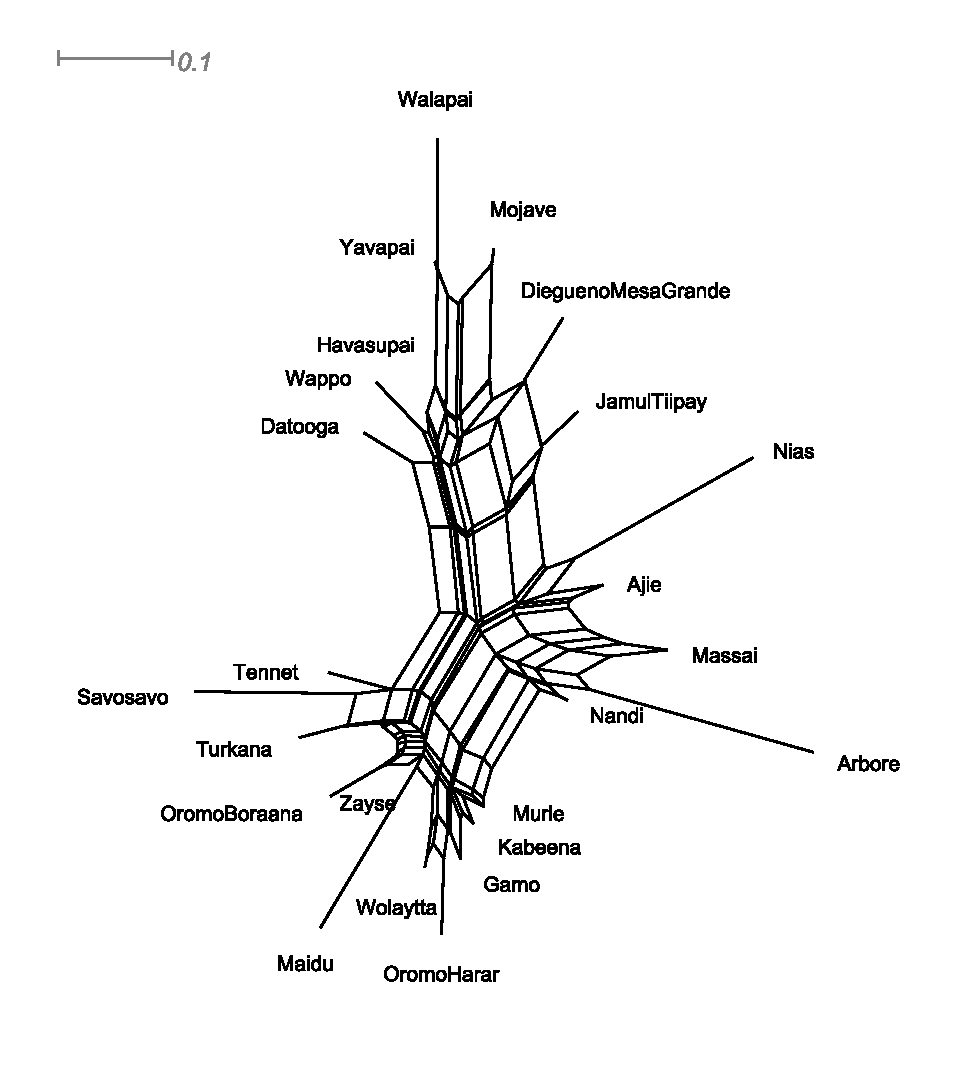
\includegraphics{languages}
}}
\caption{Similarity network of the languages studied}\label{NetLang}
\end{figure}

The next network groups the data by languages (see Figure~\ref{NetLang}). 
The most salient subdivision of the language network is the one between the Yuman languages and Wappo\il{Wappo}, which form a North-West American subtype of marked"=S, and the rest of the network. 
The other American language of this sample, i.e. Maidu\il{Maidu}, does not belong to this typological subgrouping. 
The Nilotic language Datooga also appears to be more similar in type to the American languages than to any other language in the sample. 
Also, the groupings within the Yuman genus are quite accurately mirrored by the network. Mesa Gande Diegue\~no\il{Diegue\~no (Mesa Grande)} and Jamul\il{Jamul Tiipay} Tiipay both belong to the Delta-California branch of Yuman, while Yavapai\il{Yavapai}, Walapai\il{Walapai} and Havasupai\il{Havasupai} form the Arizona Pai branch. 
Mojave\il{Mojave}, which is located between these two groups in the network, belongs to the River Yuman branch. 
Other genealogical groupings that are represented in the network are the Afro-Asiatic languages from the Omotic and Eastern Cushitic branch (except Arbore\il{Arbore}, which is separated from its related languages).
Even though these languages are found in an continuous segment of the network (with intervening Maidu\il{Maidu}, which exhibits the most areally atypical pattern of the sample), they do not form a clear branch structure that would set them off from other languages. 
However, there is a distinct African subgroup, although it is not limited to the languages of the Afro-Asiatic family. 
If one adds the non-related Surmic languages (Murle\il{Murle} and Tennet\il{Tennet}) and the Nilotic language Turkana\il{Turkana} of the Nilo-Saharan family as well as Maidu\il{Maidu} and Savosavo\il{Savosavo}, a distinct group separated from the remaining languages by a branch-like structure can be identified. 

The Austronesian languages Aji\"e\il{Aji\"e} and Nias\il{Nias} are located in adjacent position at the border between the North American and African languages, but like the Afro-Asiatic language, they do not form an individual branch structure.
The Nilotic languages, on the other hand, are scattered all over the network and so do not form any continuous subsection of the network.
This genus has already been shown to be the most divergent at the tabular ranking in the previous section.

\begin{figure}[h,t,b,p] \centering \resizebox{\textwidth}{!}{\fbox{
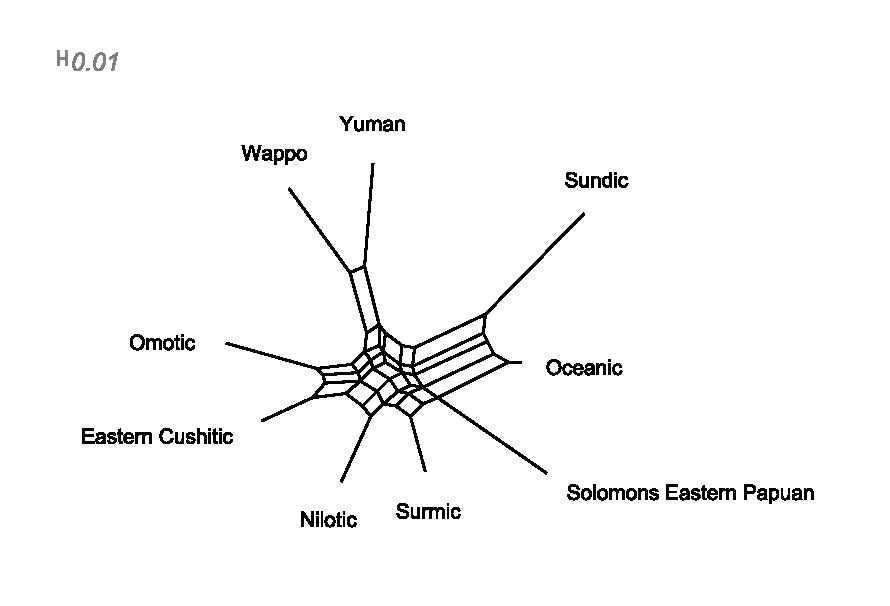
\includegraphics{genus}
}}
\caption{Similarity network of the genera studied}\label{NetGenus}
\end{figure}

Finally the data is grouped by genus (Figure~\ref{NetGenus}). 
For this network, Maidu\il{Maidu} (Maidu\il{Maidu}an) has been eliminated.
It has already been noted that Maidu\il{Maidu} behaves quite unusual compared with the marked"=S languages in its macro-area.
Also compared with the total set of marked"=S languages, it stands out by employing the S-case almost like would be expected from a regular nominative"=accusative language. 
Other than the Omotic marked"=S languages, which also make wide use of the S-case, and which have overtly coded forms for both S-case and zero-case, on the formal level Maidu\il{Maidu} is a typical marked"=S language. 

Also\is{multidimensional scaling|(} when analyzing the language-internal grouping of uses in the Maidu\il{Maidu} data, the picture is confusing. 
The semantic map in Figure~\ref{maidu} visualizes the use of S-case (red/subj), zero-case (blue/zero) and other case-forms (black/other) in Maidu\il{Maidu}.
\footnote{Again, I have to thank Michael Cysouw. This time for producing and sharing this semantic map.}  
The arrangement of the roles is derived from the usage of these case-forms for the individual roles across all languages of the sample via multidimensional scaling (MDS). 
Semantic maps derived through MDS and how they can be used to analyze and understand the nature of linguistic meanings are discussed by \citet{Cysouw:2010}.
While the other languages use the individual case-forms for continuous parts of the semantic map (or at least only one case-form shows discontinuous usage), Maidu\il{Maidu} rather constitutes a semantic patchwork.\is{multidimensional scaling|)}  

Furthermore, including Maidu\il{Maidu} into the genus level network gives no clear picture. 
If one excludes this data, the genealogical and areal groupings come out quite nicely, as demonstrated in Figure~\ref{NetGenus}.
The North American languages have already formed a distinct subgroup on the language level. 
Not surprisingly, Yuman and Wappo\il{Wappo} also form the most clear subgrouping in this graph. 
They branch off almost tree-like from the other genera. 
The African genera also form a distinct area of the network, and especially the Afro-Asiatic genera Omotic and Eastern Cushitic even form a small separate branch. 
The two Nilo-Saharan genera, Nilotic and Surmic, are adjacent to one another, though they form no branch-like structure. 
The Austronesian genera, Sundic and Oceanic, also from a separate branch of the network (though the branching is not particularly strong) with Solomons East Papuan, the other Pacific genus, in adjacent position.\is{phylogenetic networks|)}

\begin{figure}[p,h,t,b] \centering \fbox{
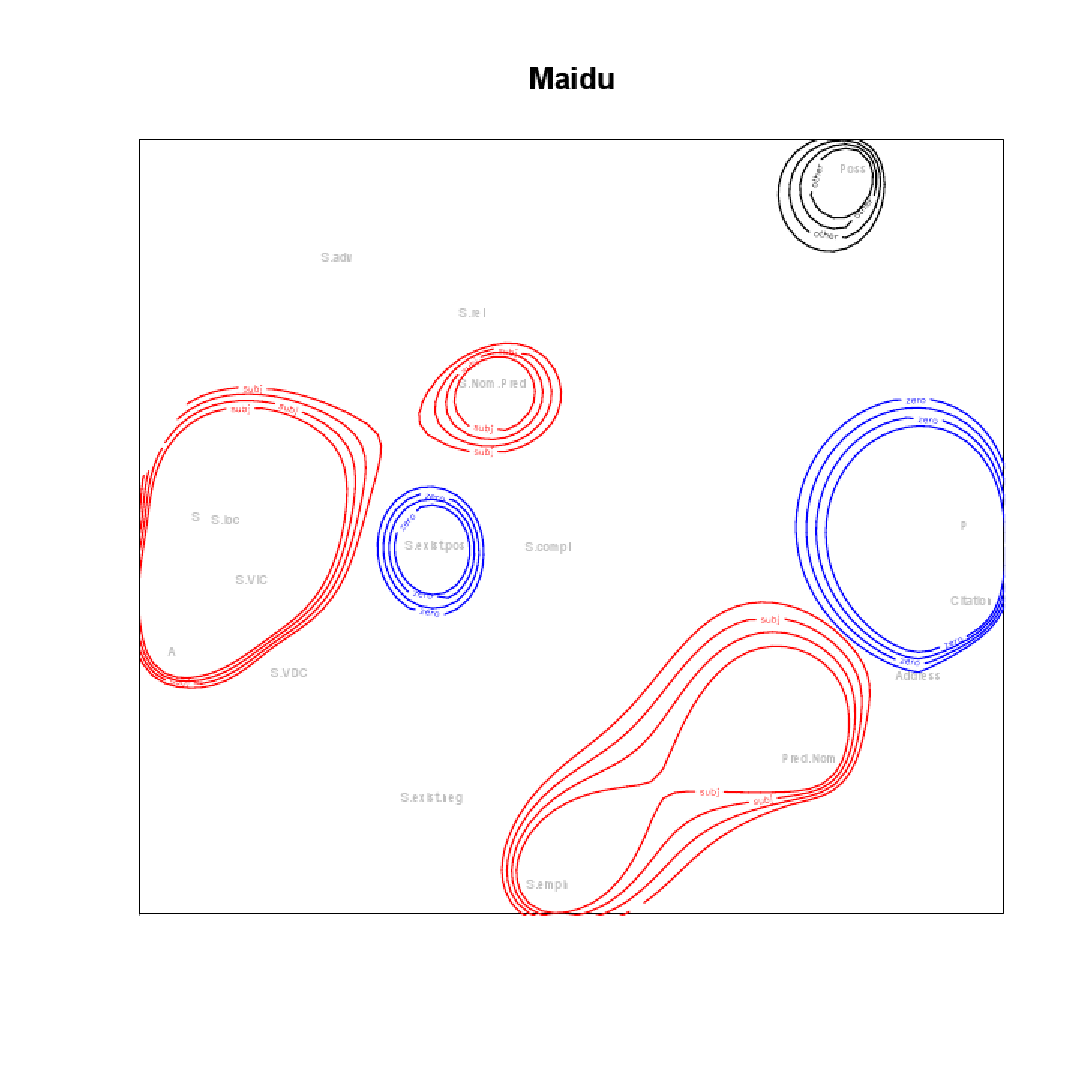
\includegraphics[scale=.65]{maidu}
}
\caption{Maidu semantic map (MDS)}\label{maidu}
\end{figure}


\section{Geographical patterns}\label{area}\is{typology!areal|(}

It has been noted several times in this study that the distribution of marked"=S languages is highly skewed in terms of geography.
North-East Africa, where the pattern is found in both the Afro-Asiatic and Nilo-Saharan family, appears to be a breeding ground for languages of this type. 
Another area in which marked"=S languages appear frequently (as compared with the overall distribution over the world) is the lower North American Pacific coast. 
The majority of marked"=S languages found in this region are closely-related with one another as they belong to one genus (i.e. Yuman). 
However, two unrelated marked"=S languages, namely Wappo\il{Wappo} and Maidu\il{Maidu}, do occur in the same macro-area.
Finally the Pacific macro-area is home to some languages of the marked"=S type. 
The three Pacific languages with the most prominent marked"=S pattern are stretched out over a quite large area. 
However, if additionally to Nias\il{Nias}, Aji\"e\il{Aji\"e} and Savosavo\il{Savosavo} the less prototypical marked"=S languages of the same region are included, such as the ones discussed in Chapter~\ref{exposed}, the Pacific exhibits an above-average concentration of marked"=S languages as well. 
In this section, I will take a closer look at the areal patterings of marked"=S languages.

\begin{figure}[h,t,b] \centering \resizebox{\textwidth}{!}{\fbox{
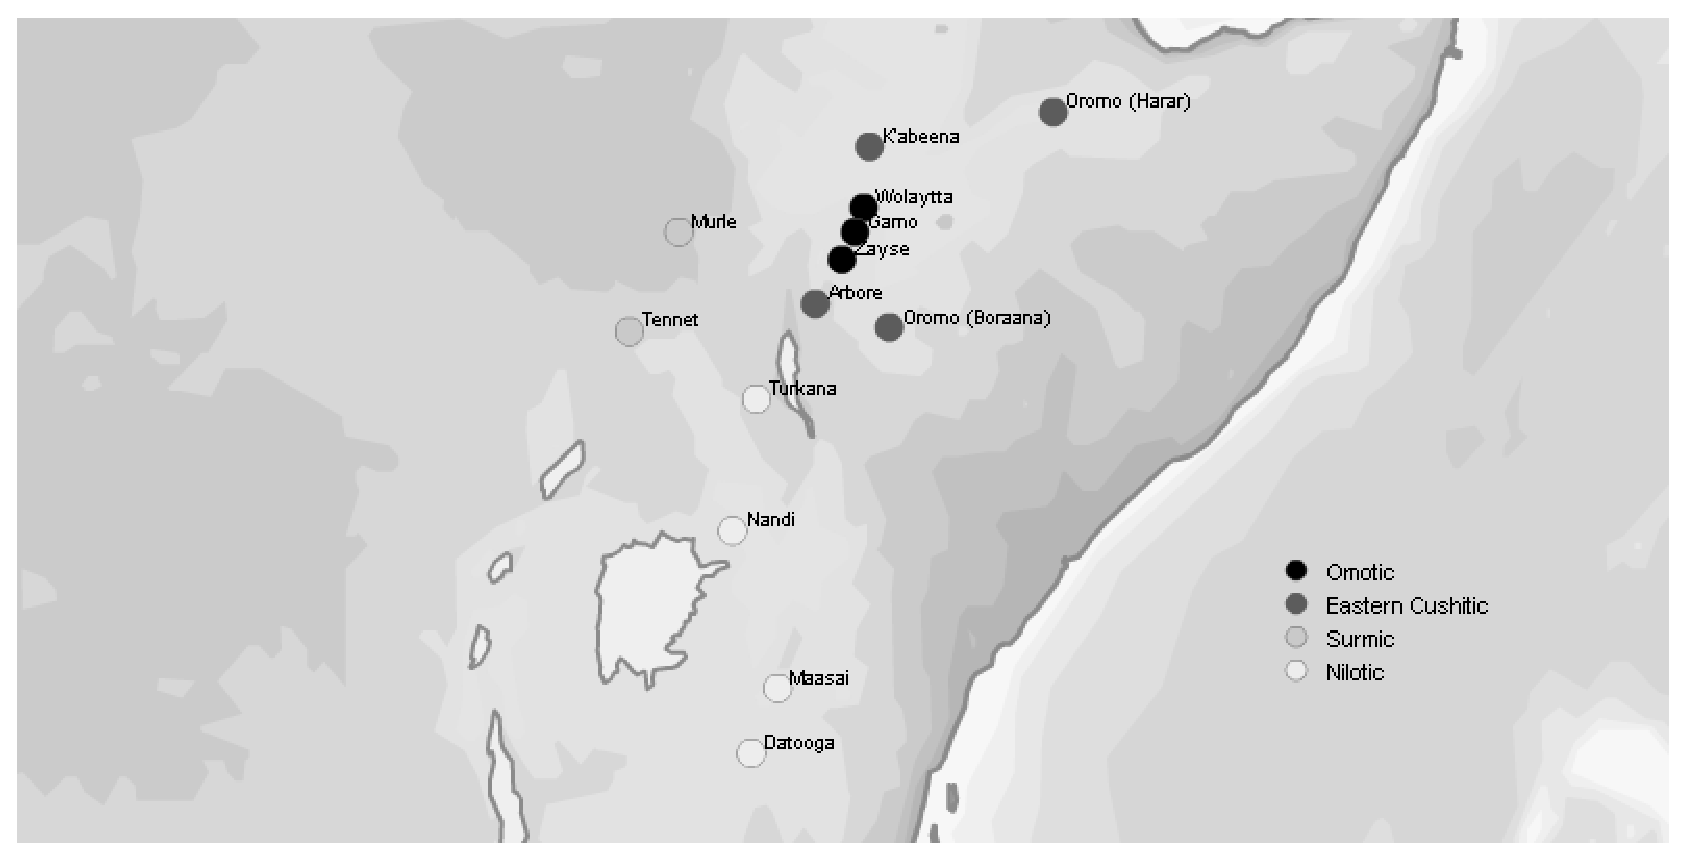
\includegraphics[scale=0.44]{MapAfrica}
}}
\caption{marked"=S languages of East Africa by genus}\label{MapAfrica}
\end{figure}

The largest number of languages in my sample is found in North-East Africa. 
In addition to the large number for the African marked"=S languages, they also exhibit genealogical diversity as they are represented by four distinct genera belonging to the Afro-Asiatic (Omotic and Cushitic) and Nilo-Saharan (Surmic and Nilotic) families (cf. Figure~\ref{MapAfrica}).
\footnote{The language Maa\il{Maa} is represented with its alternative name Maasai in the map.} 
Marked"=S patterns have been reported from other genera of this area, but the data available for them was not suitable to include in this study. 
Areal influence is often proposed as an explanation if a certain linguistic pattern is found in a group of geographically adjacent but non-related languages, even more so if the respective pattern is rare on a world-wide basis.
The locus of the African marked"=S languages has been suggested as a linguistic area on several occasions.
\citet{Gueldemann:2005}\is{typology!areal!Ethiopian language area|(} describes a pattern of forming complex predicates through a special type of auxiliary that is uniquely found in the region referred to as Chad-Ethiopia macro-area. 
This region has been described as a linguistic area in earlier work by \citet{Greenberg:1983}, \citet{Ferguson:1976} and \citet{Heine:1976}, though the name and exact boundaries of the supposed area differ between the authors.
However, the existence of an `Ethiopian language area' is disputed by \citet{Tosco:2000}. 
Yet, his main argument is not that there has not been linguistic contact between unrelated languages in this area, but that the influence has been unidirectional. 
He lists multi-directional influence and divergence towards a common model as defining criteria for linguistic areas.\is{typology!areal!Ethiopian language area|)} 
The network in Figure~\ref{NetLang} has shown that the African languages do not group according to their genealogical affiliations in most cases with respect to the roles studied here. 
Only the Omotic languages in combination with most Cushitic languages do occur in adjacent position. 
However, they do not exhibit any clear tree-like branching from the other African languages (and also the Pacific languages plus Maidu\il{Maidu}). %THis might change
Instead they all are of the same general type, with the exclusion of Datooga, which is more similar to the North American languages in its behavior. 
Notably Datooga, which is the least typical African marked"=S language, is spoken at the periphery of the geographical region these languages cover.
In addition, Datooga and Maa\il{Maa} are the two African languages that make the widest use of the zero-case and thus have been shown to behave quite differently than the two other Nilotic languages in the sample in Table~\ref{SumRoleLang}. 
Indeed, Maa\il{Maa} is the language that is spoken closest to Datooga, though it is not the language which is related most closely in terms of genealogy. 


\begin{figure}[h,t,b] \centering \resizebox{\textwidth}{!}{\fbox{
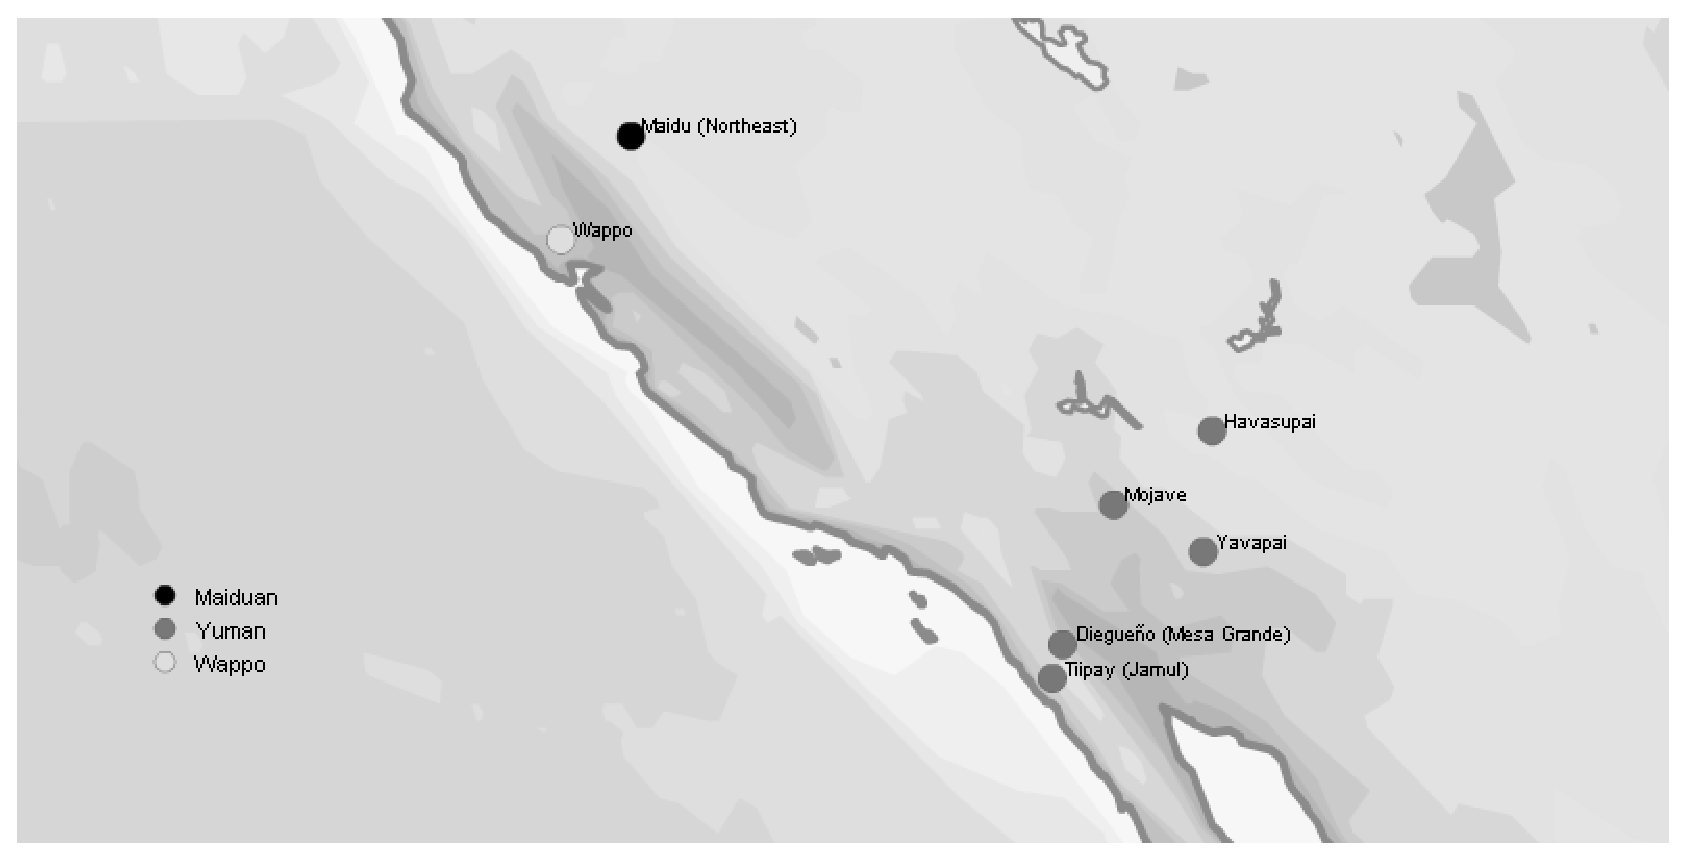
\includegraphics[scale=0.44]{MapNA}}
}\caption{marked"=S languages of North-West America by genus}\label{MapNA}
\end{figure}

The second larger grouping of marked"=S languages is found in North-West America. 
These languages are far less genealogically diverse than their African counterparts. 
The majority of languages belongs to the Yuman genus, which is completely of the marked"=S type, except for only one language, namely Kiliwa \citep{Mixco:1965}, which is also seen as the language that first branched of within the genus \citep{Joel:1998}. %find better source
Apart from the Yuman languages, two other marked"=S languages of this region are studied here. 
Wappo\il{Wappo} and Maidu\il{Maidu} are both located quite a stretch to the North from the Yuman languages (cf. Figure~\ref{MapNA}), so that the American languages do not form a contiguous area.
Apart from the close geographical distance between Maidu\il{Maidu} and Wappo\il{Wappo}, these two languages do not show a similar linguistic behavior. 
Wappo\il{Wappo} rather conforms to the most frequent type of American marked"=S languages with the Yuman languages. 
Maidu\il{Maidu} does not show any similarities to this type.
In the network in Figure~\ref{NetLang}, it is located somewhere between Omotic and some Cushitic languages, the main similarity to which is Maidu\il{Maidu}'s equally high percentage of S-case use.
For the Yuman languages of North America, genealogy is probably the main factor behind their common typological profile with respect to their marked"=S case-system.
Wappo\il{Wappo} is a language of the same greater area which is not related to this genus. 
However, it has a typological profile similar to the Yuman languages.
No contact history between the Yuman languages and Wappo\il{Wappo} is known and the geographical distance between the languages (in addition to the large number of intervening languages) makes this scenario not very likely. 
However, one should not rule out that in prehistoric times both Wappo\il{Wappo} and the Yuman languages were part of a larger linguistic area in which marked"=S languages were more abundant. 
If one takes this scenario seriously, Maidu\il{Maidu}, which is located more closely to Wappo\il{Wappo}, could also have been a part of this area. 
Still, Maidu\il{Maidu}'s marked"=S system is distinct from the other North American languages. 
So the system either must have radically changed after the hypothetical period of intense contact with other languages of the marked"=S type, or it could be a development independent of contact with languages that exhibit the typical North American type of marked"=S.

\begin{figure}[h,t,b] \centering \resizebox{\textwidth}{!}{\fbox{
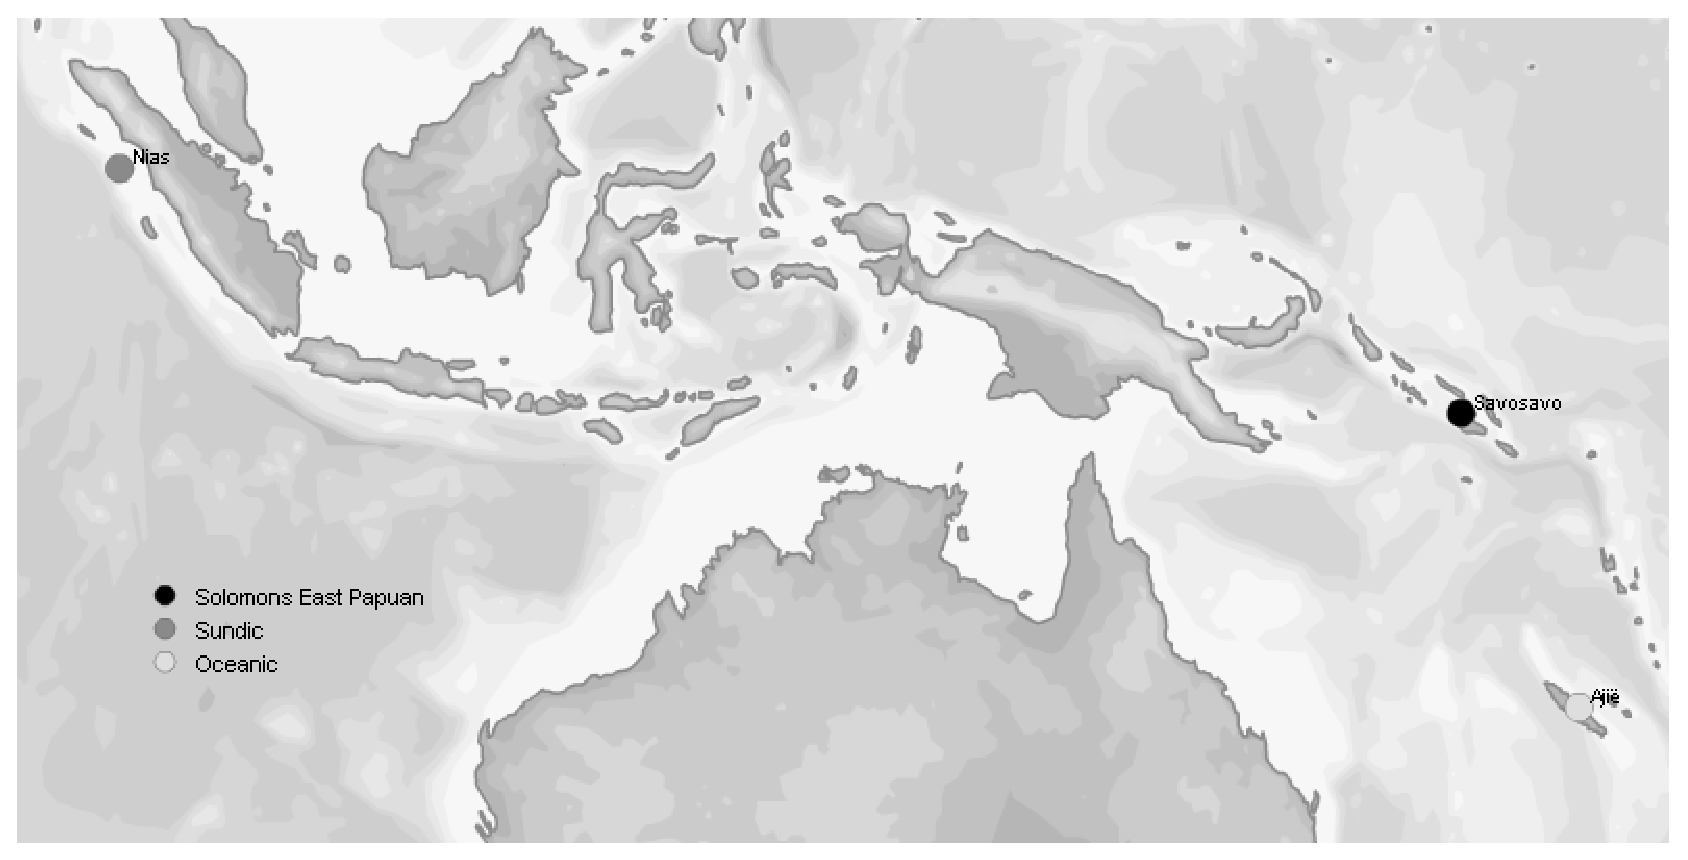
\includegraphics[scale=0.44]{MapPac}
}} \caption{Marked"=S languages of the Pacific by genus}\label{MapPac}
\end{figure}

Finally, the sample included three marked"=S languages from the larger Pacific region. 
Comparing their distribution (cf. Figure~\ref{MapPac}), it becomes clear that arguing for contact between these languages as source for the marked"=S pattern would be rather difficult given that these three languages are stretched out from the West Coast of Sumatra to the Solomon Islands and down to New Caledonia. 
In addition, the genealogical relation between these languages is very distant (Nias\il{Nias} and Aji\"e\il{Aji\"e} belong to different genera of the Austronesian family) or non-existent (as between Savosavo\il{Savosavo} and the other two languages). 
In between the three languages studied in detail lies the entire Indonesian Archipelago including all of Papua as well as large stretches of the Pacific Ocean.
However, within this area there are a number of languages exhibiting a pattern that resembles the marked"=S languages in some respect. 
I have discussed this pattern, which consists of overt subject-marking only in certain, mostly emphatic\is{emphatic subject}, contexts, in Chapter~\ref{emphaticS}.
Adding these languages to the map, as done in Figure~\ref{MapPacAll}, at least the Eastern half of the region pictured here gets closer resemblance to an geographically contiguous area, which includes Savosavo\il{Savosavo} and Aji\"e\il{Aji\"e} at its periphery. 

\begin{figure}[h,t,b] \centering \resizebox{\textwidth}{!}{\fbox{
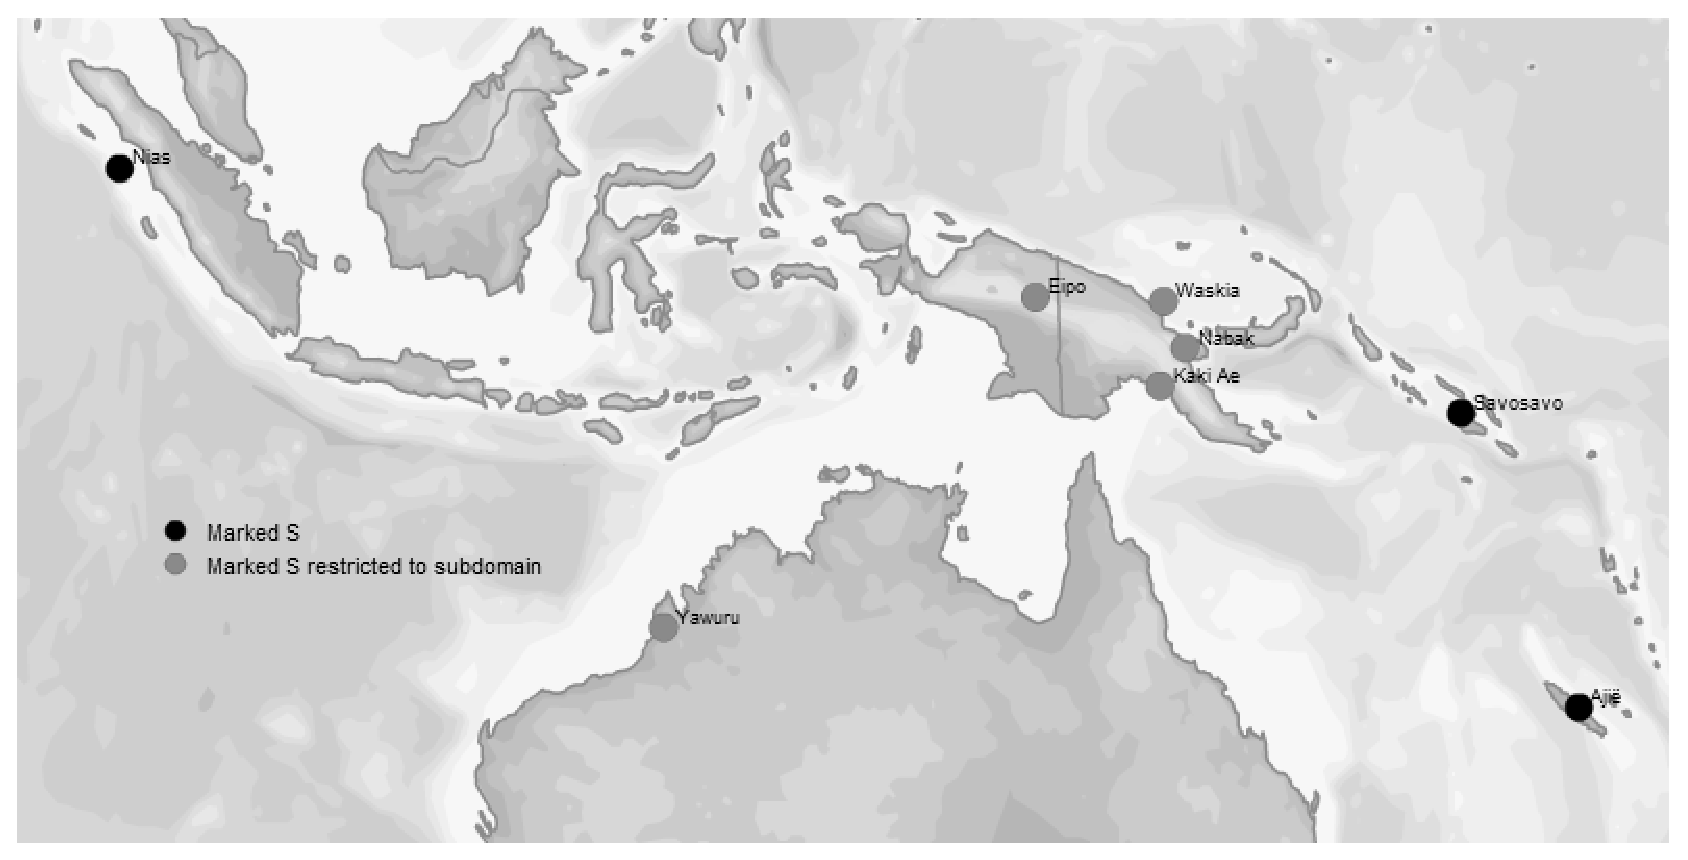
\includegraphics[scale=0.44]{MapPacAll}}
} \caption{Marked"=S languages of the Pacific including full and restricted patterns}\label{MapPacAll}
\end{figure}\is{typology!areal|)}


\section{Summary}\label{sumtyp}

In this chapter, I have presented a summary of the data gathered through Chapters~\ref{nompred}--\ref{extrasyn}. 
The micro-alignment approach I have chosen for the investigation of marked"=S languages consists of collecting data on the case-marking patterns for a number of roles. 
These roles were selected from several contexts that include a subject-like\is{grammatical relations|subject} role (such as nominal predications or existentials\is{existential predication}), or roles that are commonly associated with the so-called `unmarked case' of standard nominative"=accusative and ergative"=absolutive languages (i.e. the nominative or absolutive respectively).
The data collected on the case-marking of these roles have been analyzed from two perspectives: from the point of view of these roles and the point of view of the languages studied.

I have demonstrated that the encoding of the roles chosen for this micro-ty\-po\-lo\-gy of the marked"=S coding-system range from (almost) exclusive encoding with the S-case to zero-coding in almost all instances. 
Roles that do not constitute any type of subject, though they have been associated with the nominative case in previous work, are especially likely to be zero-coded. 
These roles are the citation\is{citation form} form and predicate nominals\is{nominal predication!predicate nominal}, as well as attributive\is{possession!attributive} possessors and terms of address\is{terms of address}. 
The latter two are, however, also frequently encoded through other overt non-S-case case-forms.

Variation is not only found between the different roles but also between the marked"=S languages. 
While some make strong use of the zero-case, others use this form more sparsely. 
Especially the Omotic languages and Maidu\il{Maidu} do not differ strongly from standard nominative"=accusative languages in the use of the S-case. 
On the other end of the hierarchy, there are the distantly related Austronesian languages Aji\"e\il{Aji\"e} and Nias\il{Nias}, a number of the North American Yuman languages and Wappo\il{Wappo} as well as the Nilotic languages Datooga and Maa\il{Maa}. 
These languages make especially wide use of the zero-case and also employ it for some types of subjects. 

Given the rarity of the phenomenon, this study has included as many languages as possible and no quotas have been set in advance, e.g. one language per genus (or other pre-defined grouping). 
In this section, in addition to the data set including the individual languages, a controlled version in which only one data point per genus was included for each role has also been presented. 
The differences between the two sets of data, the language and genus level, have been very small. 

Also, two different encodings for the case-marking have been employed for the data. 
These two codings roughly correspond to the weak and strong interpretation of K\"onig's (\citeyear{Koenig:2006}) functional marked"=S hypothesis. 
The weak version states that the zero-case should be employed in more contexts in marked"=S languages than the overtly coded S-case. 
To analyze this version of the hypothesis the data has been coded according to whether a role is marked with the zero-case, S-case or another case-form. 
The strong version of the hypothesis states that the zero-case should be more frequent than any other type of encoding, respectively the data has been coded as zero-coding and overt coding to test this claim.
The differences between the two types of coding have been minor and are mostly restricted to non-subject roles such as attributive\is{possession!attributive} possessors.
Most languages either choose the zero-case or the S-case for the majority of roles investigated in this study.

In addition, the data have been analyzed in form of phylogenetic networks produced through the NeighborNet algorithm. 
The networks in general confirm the picture gained from the depiction in the form of tables ranked by percentage of use of the individual case-forms.
The roles appear to show a clear separation between those that constitute some kind of subject and those that have different, mostly non-clause level, functions. 
The data on the languages do not show any neat subtypes of marked"=S languages apart from the grouping of the Yuman languages and Wappo\il{Wappo}.
The data on the genus level, meanwhile, produced an accurate picture of the genealogical and areal groupings of languages. 
However, one language, namely Maidu\il{Maidu}, had to be excluded in order to arrive at this neat depiction. 

Geographically, the languages of the sample can bee grouped as belonging to three marco-areas: North-Eastern Africa, the North American West Coast, and the Pacific. 
The languages of North America, to the exclusion of Maidu\il{Maidu}, do form the most distinct subtype in all analyses of the data. These languages mostly belong to the Yuman genus. 
However, non-related Wappo\il{Wappo} also behaves quite similarly to the Yuman languages. The other type of marked"=S languages against which the American type can be set off consists mostly of the African languages. 
The Afro-Asiatic languages, especially of the Omotic genus, are another potential subtype of marked"=S languages. 
However, these languages do not form as distinct a subtype branching off from other languages as does the American type. 
Nilo-Saharan, the other African language family, generally tends to cluster around the Afro-Asiatic languages. 
These languages do not provide a legitimate grouping with each other, especially the languages of the Nilotic genus do not exhibit a uniform behavior according to the methods of comparison employed. 
Languages of the Pacific are too few within the sample to make any strong claims about a distinct type. 
Yet, the two Austronesian languages Aji\"e\il{Aji\"e} and Nias\il{Nias} behave quite similarly to one another in the different modes of analysis used in this chapter.  

